


\section{The Design and Implementation of Torta}

\begin{figure*}[h!]
%\vspace{20em}
\centering
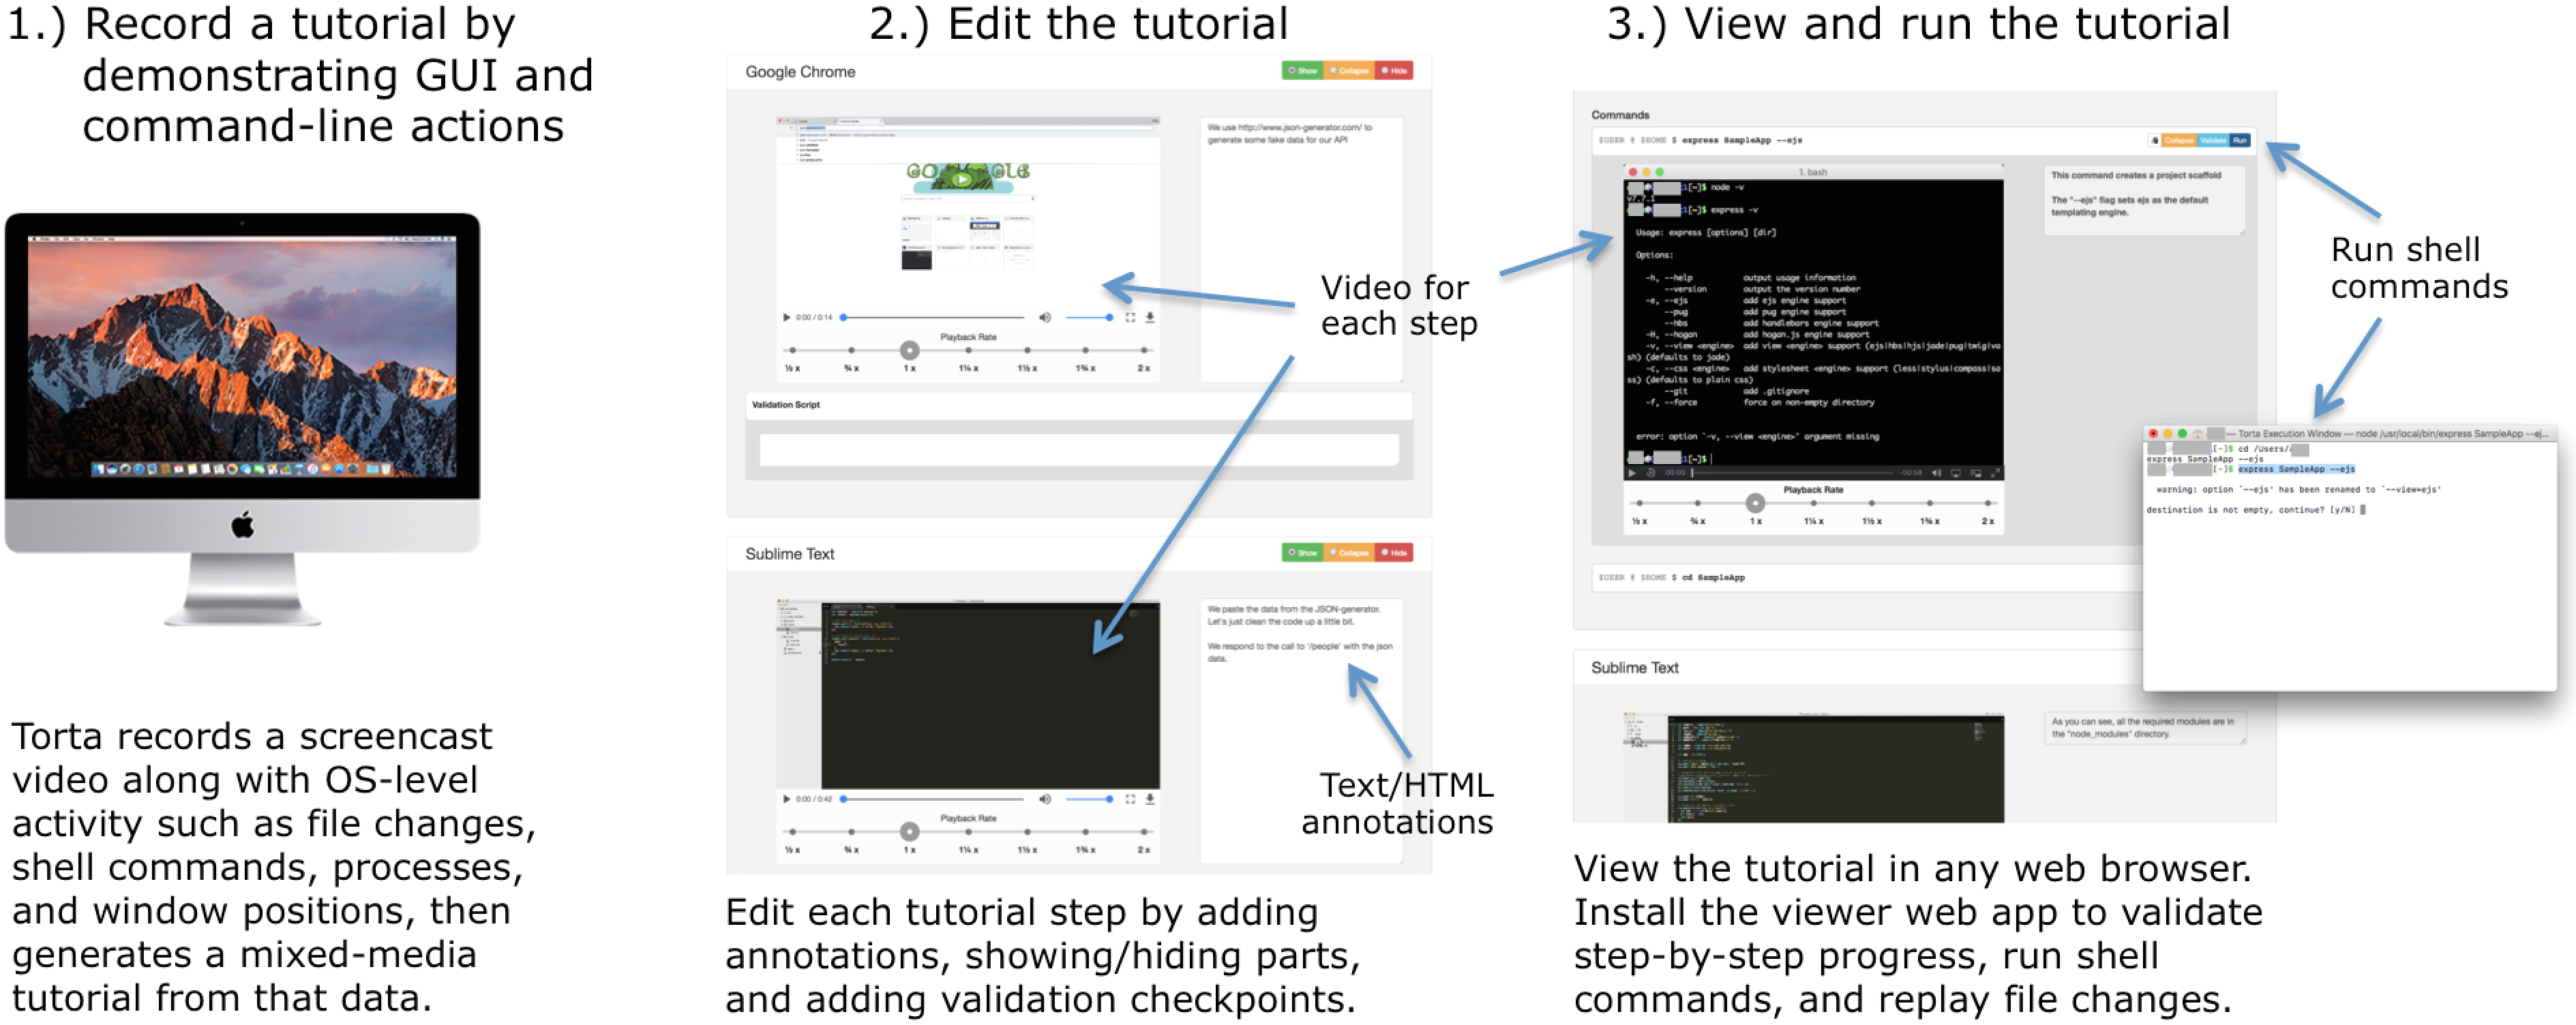
\includegraphics[width=0.98\textwidth]{figures/torta/torta-overview.png}

%\vspace{0.5em}
\caption{Torta allows macOS users to create mixed-media tutorials
by demonstration, and then edit, view, and run those tutorials in a web
browser.}

\label{fig:torta-overview}
\end{figure*}

Torta consists of three components: a tutorial recorder, editor, and
viewer (\fig{fig:torta-overview}). We now describe each in turn.


\subsection{Tutorial Recorder}

Torta's recorder allows the user to record a tutorial just as easily as
recording a screencast video (Design Goal D1).
%
Our prototype is implemented for macOS using AppleScript, Python, Bash,
and DTrace~\cite{Cantrill2004} scripts to perform OS-level activity tracing. It
should be straightforward to port this OS-wide tracing-based approach to other
operating systems.

%such as
%Windows and Linux-based systems since they offer similar kinds of
%scripting and tracing features.

When the user wants to start recording a tutorial, they activate Torta
by running a terminal command, which immediately launches a set of
activity tracers. The user then records their tutorial by simply
demonstrating actions on their computer, and the tracers log the
following data in the background:

\begin{itemize}\itemsep0pt

\item \textbf{Screencast video recorder}: Torta uses Apple's built-in
Quicktime app to record a standard full-screen screencast video with
audio narration and mouse clicks visualized.

\item \textbf{Foreground GUI window monitor}: The position and
dimensions of the user's current foreground GUI window are logged once
per second, along with the process ID of the program that owns the
current foreground window.

\item \textbf{Keystroke logger}: All user keystrokes are logged.

%using Apple's {\small \texttt{CGEventCallback}} events.

\item \textbf{Shell command logger}: The contents of all terminal
commands run in any shell are logged and timestamped. The current
working directory, username, and environment variables used for running
each command are also logged. Our current logger works for Bash (the
default on macOS) and Zsh, but can be easily extended to other custom
shells.

\item \textbf{Filesystem activity tracer}: Torta uses DTrace~\cite{Cantrill2004} to record
a subset of system calls that access the filesystem. Specifically, it
logs the timestamps, owner process IDs, and parameters of the following
filesystem-related system calls: {\small \texttt{open()}}, {\small
\texttt{write()}}, {\small \texttt{close()}}, {\small
\texttt{rename()}}, and {\small \texttt{unlink()}} (for opening, writing
to, closing, renaming, and deleting files, respectively).
Torta makes a timestamped backup copy of each affected file after the
respective system call is run. This feature is useful for saving all versions of
files that users edit within interactive applications such as text
editors, IDEs, or Photoshop: Each time the user presses ``Save" within the app, a
{\small \texttt{write()}} system call occurs, and Torta saves a backup
copy\rev{, which lets it later display diffs}.

\item \textbf{OS process tree logger}: Torta logs the command names,
start/end timestamps, process IDs (PIDs), and parent process IDs (PPIDs)
of all OS processes launched after the user activates Torta. This log
serves two purposes: First, it filters the system call trace (see above)
to consider only processes that launched \emph{after} the user activated Torta,
which eliminates the noise from dozens of irrelevant system-wide
processes previously running on the user's machine. Second, it is
necessary for linking the system call trace to foreground GUI windows.
Here is why: Many interactive apps adopt a multi-process model for
robustness. For instance, Google Chrome launches one OS process per
browser tab, and text editors such as Sublime Text launch one OS process
per text editor tab along with a separate process for the GUI. Thus, the
process that owns the Sublime Text foreground GUI window is \emph{not}
the process that makes the {\small \texttt{write()}} system calls to
save the user's files. Torta can use the OS process tree of
PIDs and PPIDs to link Sublime Text's user-initiated file save events with its GUI
window, since they are owned by sibling processes.

\end{itemize}


\begin{figure}[h!]

\centering
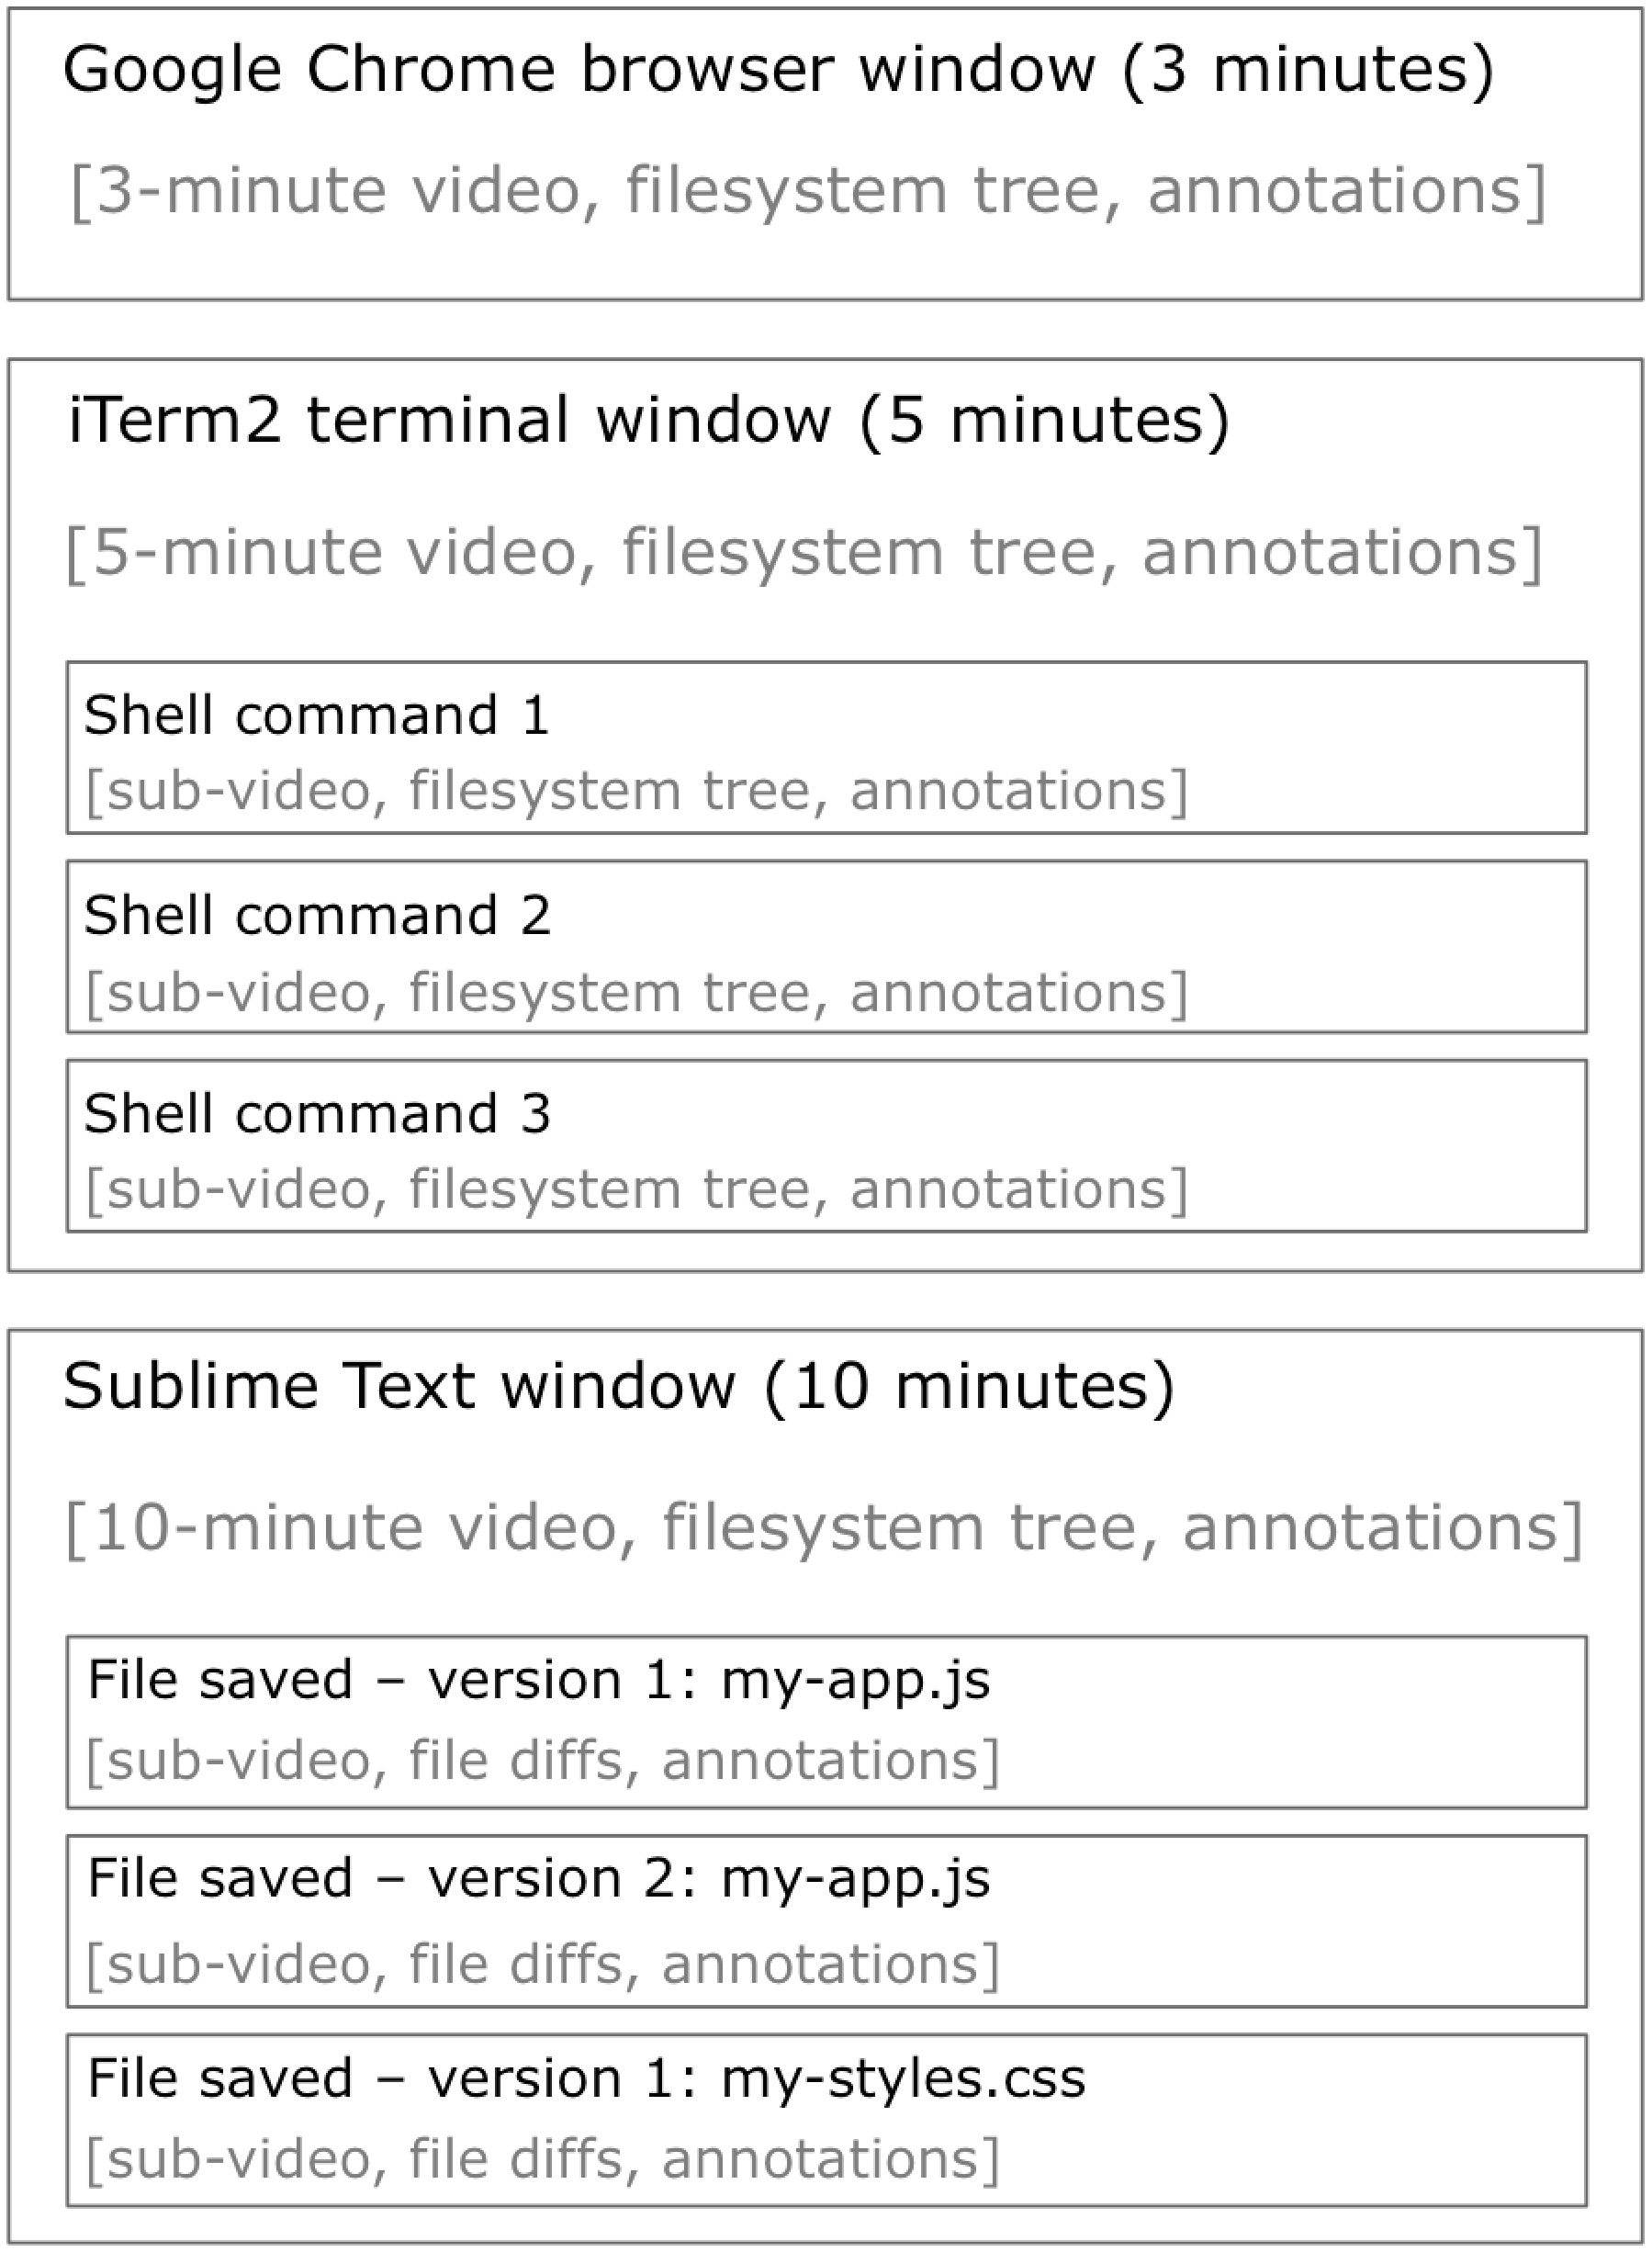
\includegraphics[width=0.5\columnwidth]{figures/torta/torta-schematic.png}

\caption{Example structure of a mixed-media tutorial generated by
Torta. Each of the three steps represents a foreground GUI window duration. There are
three sub-steps within the terminal and IDE windows.}

\label{fig:torta-schematic}
\vspace{-1em} % stent
\end{figure}


\begin{figure*}[h!]

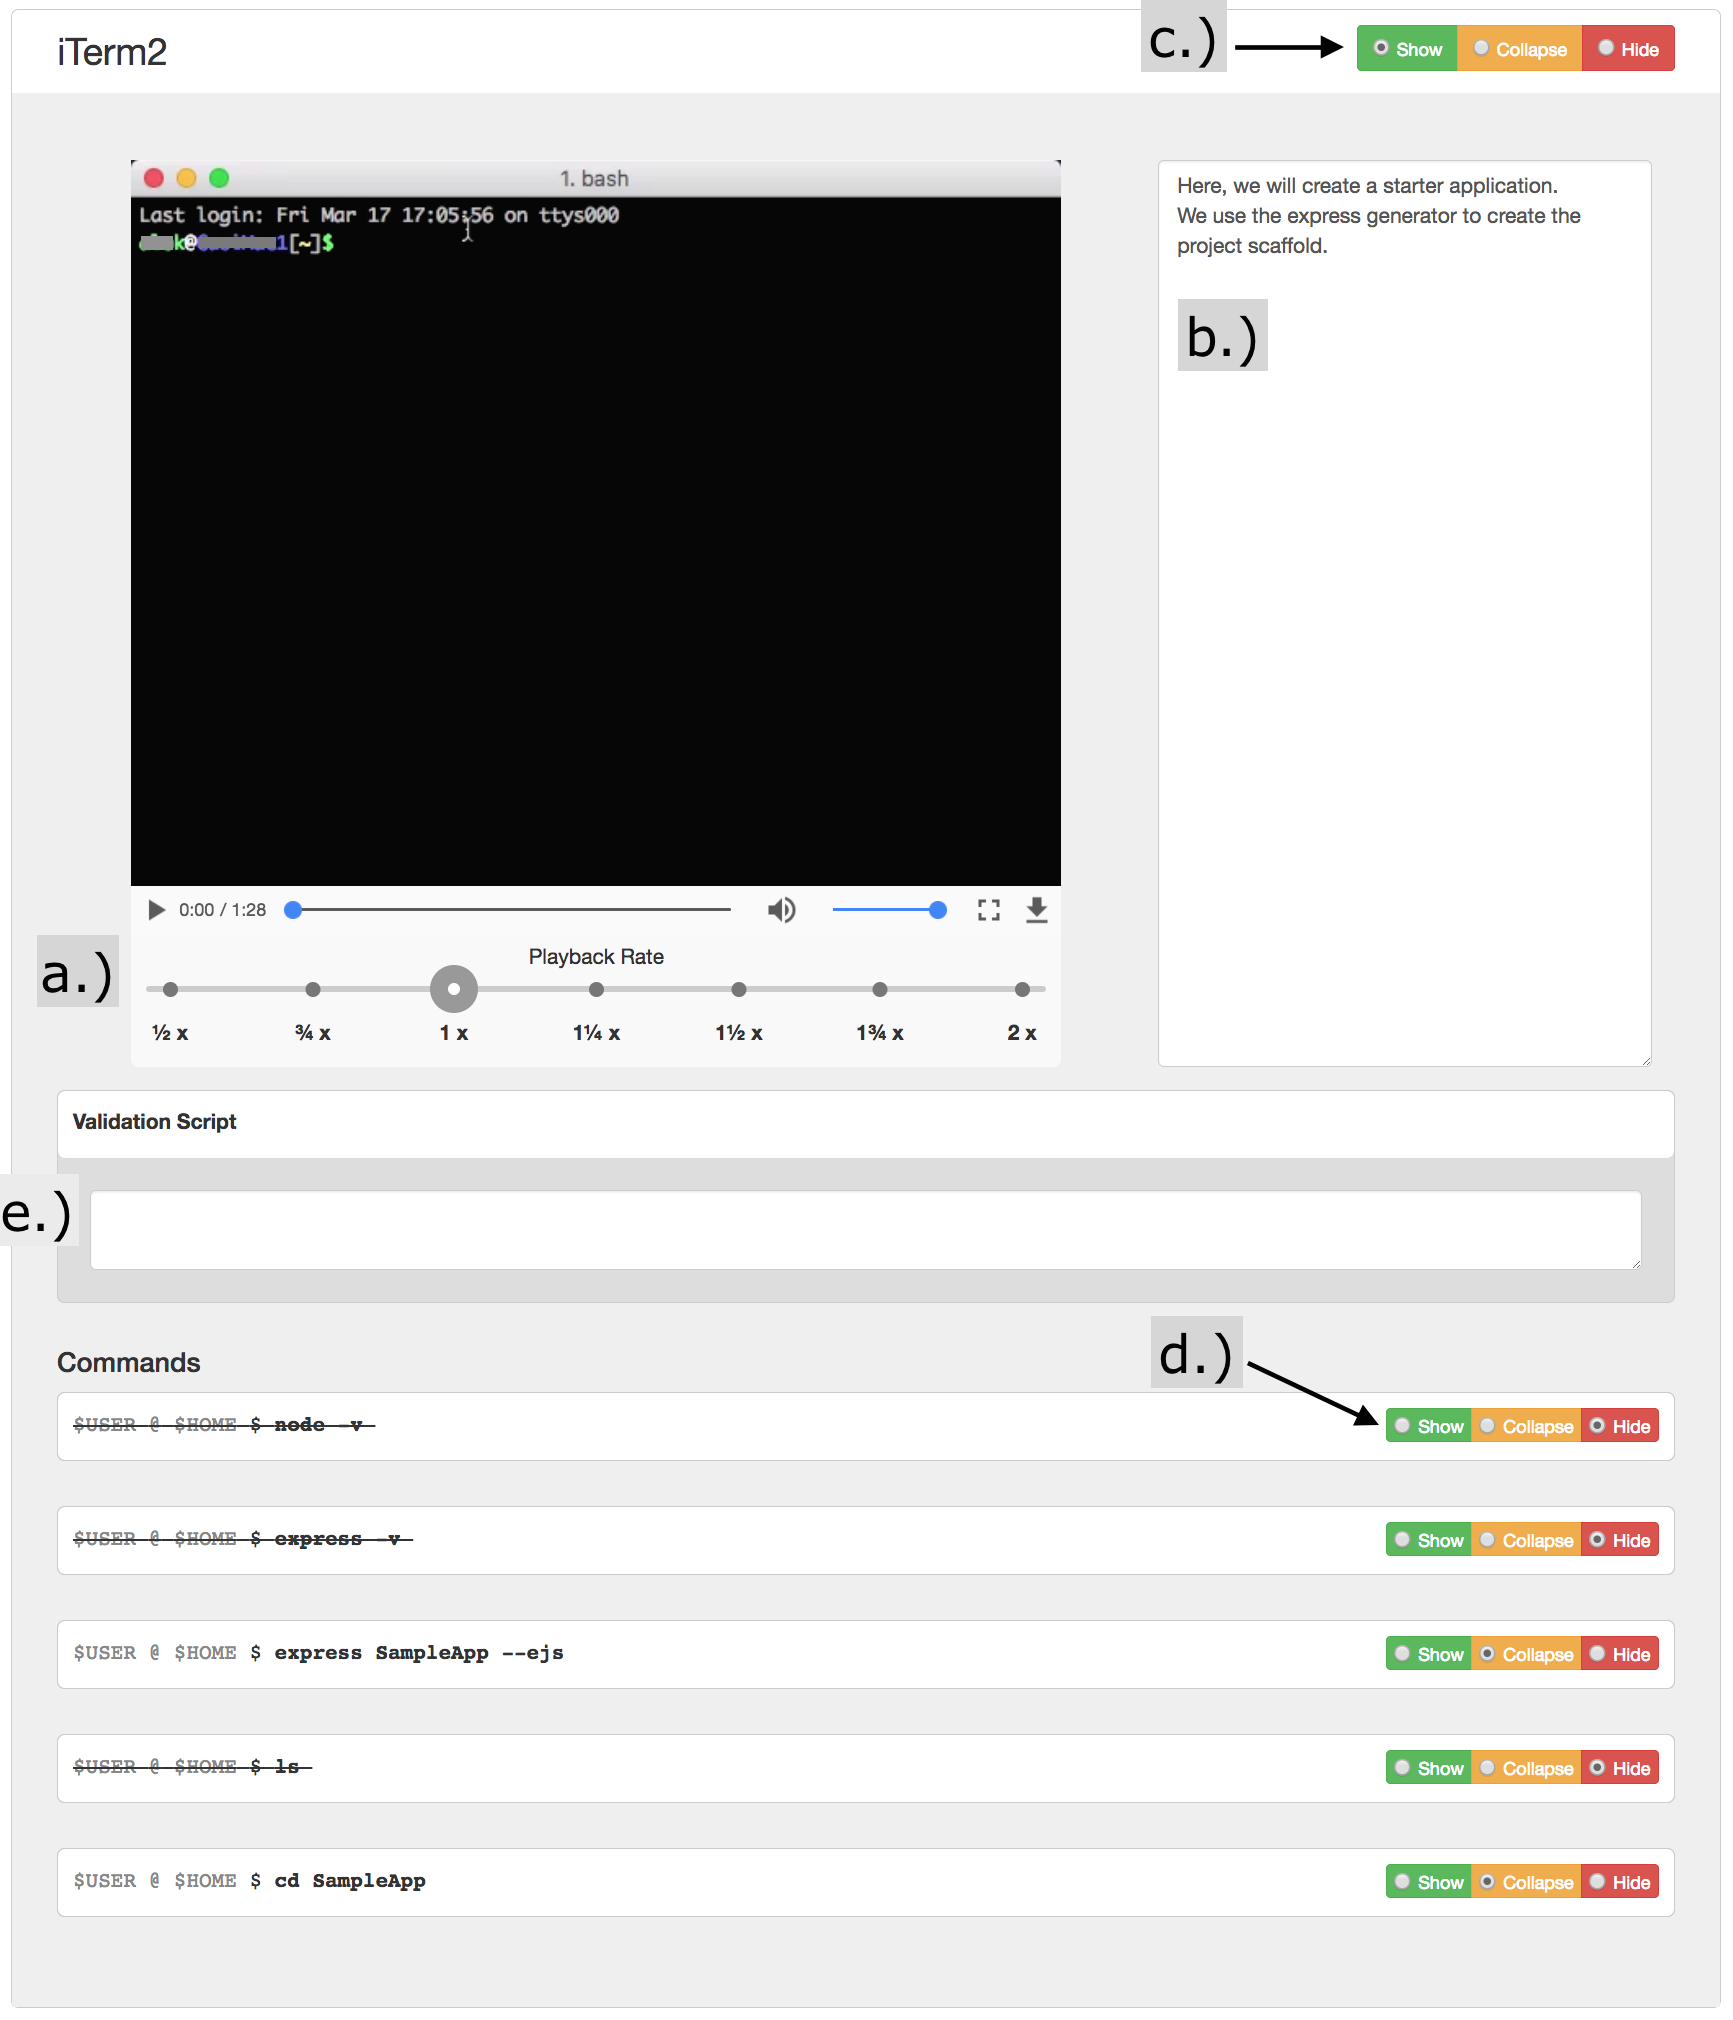
\includegraphics[width=0.488\textwidth]{figures/torta/editor-iterm2.png}
\hspace{6em}
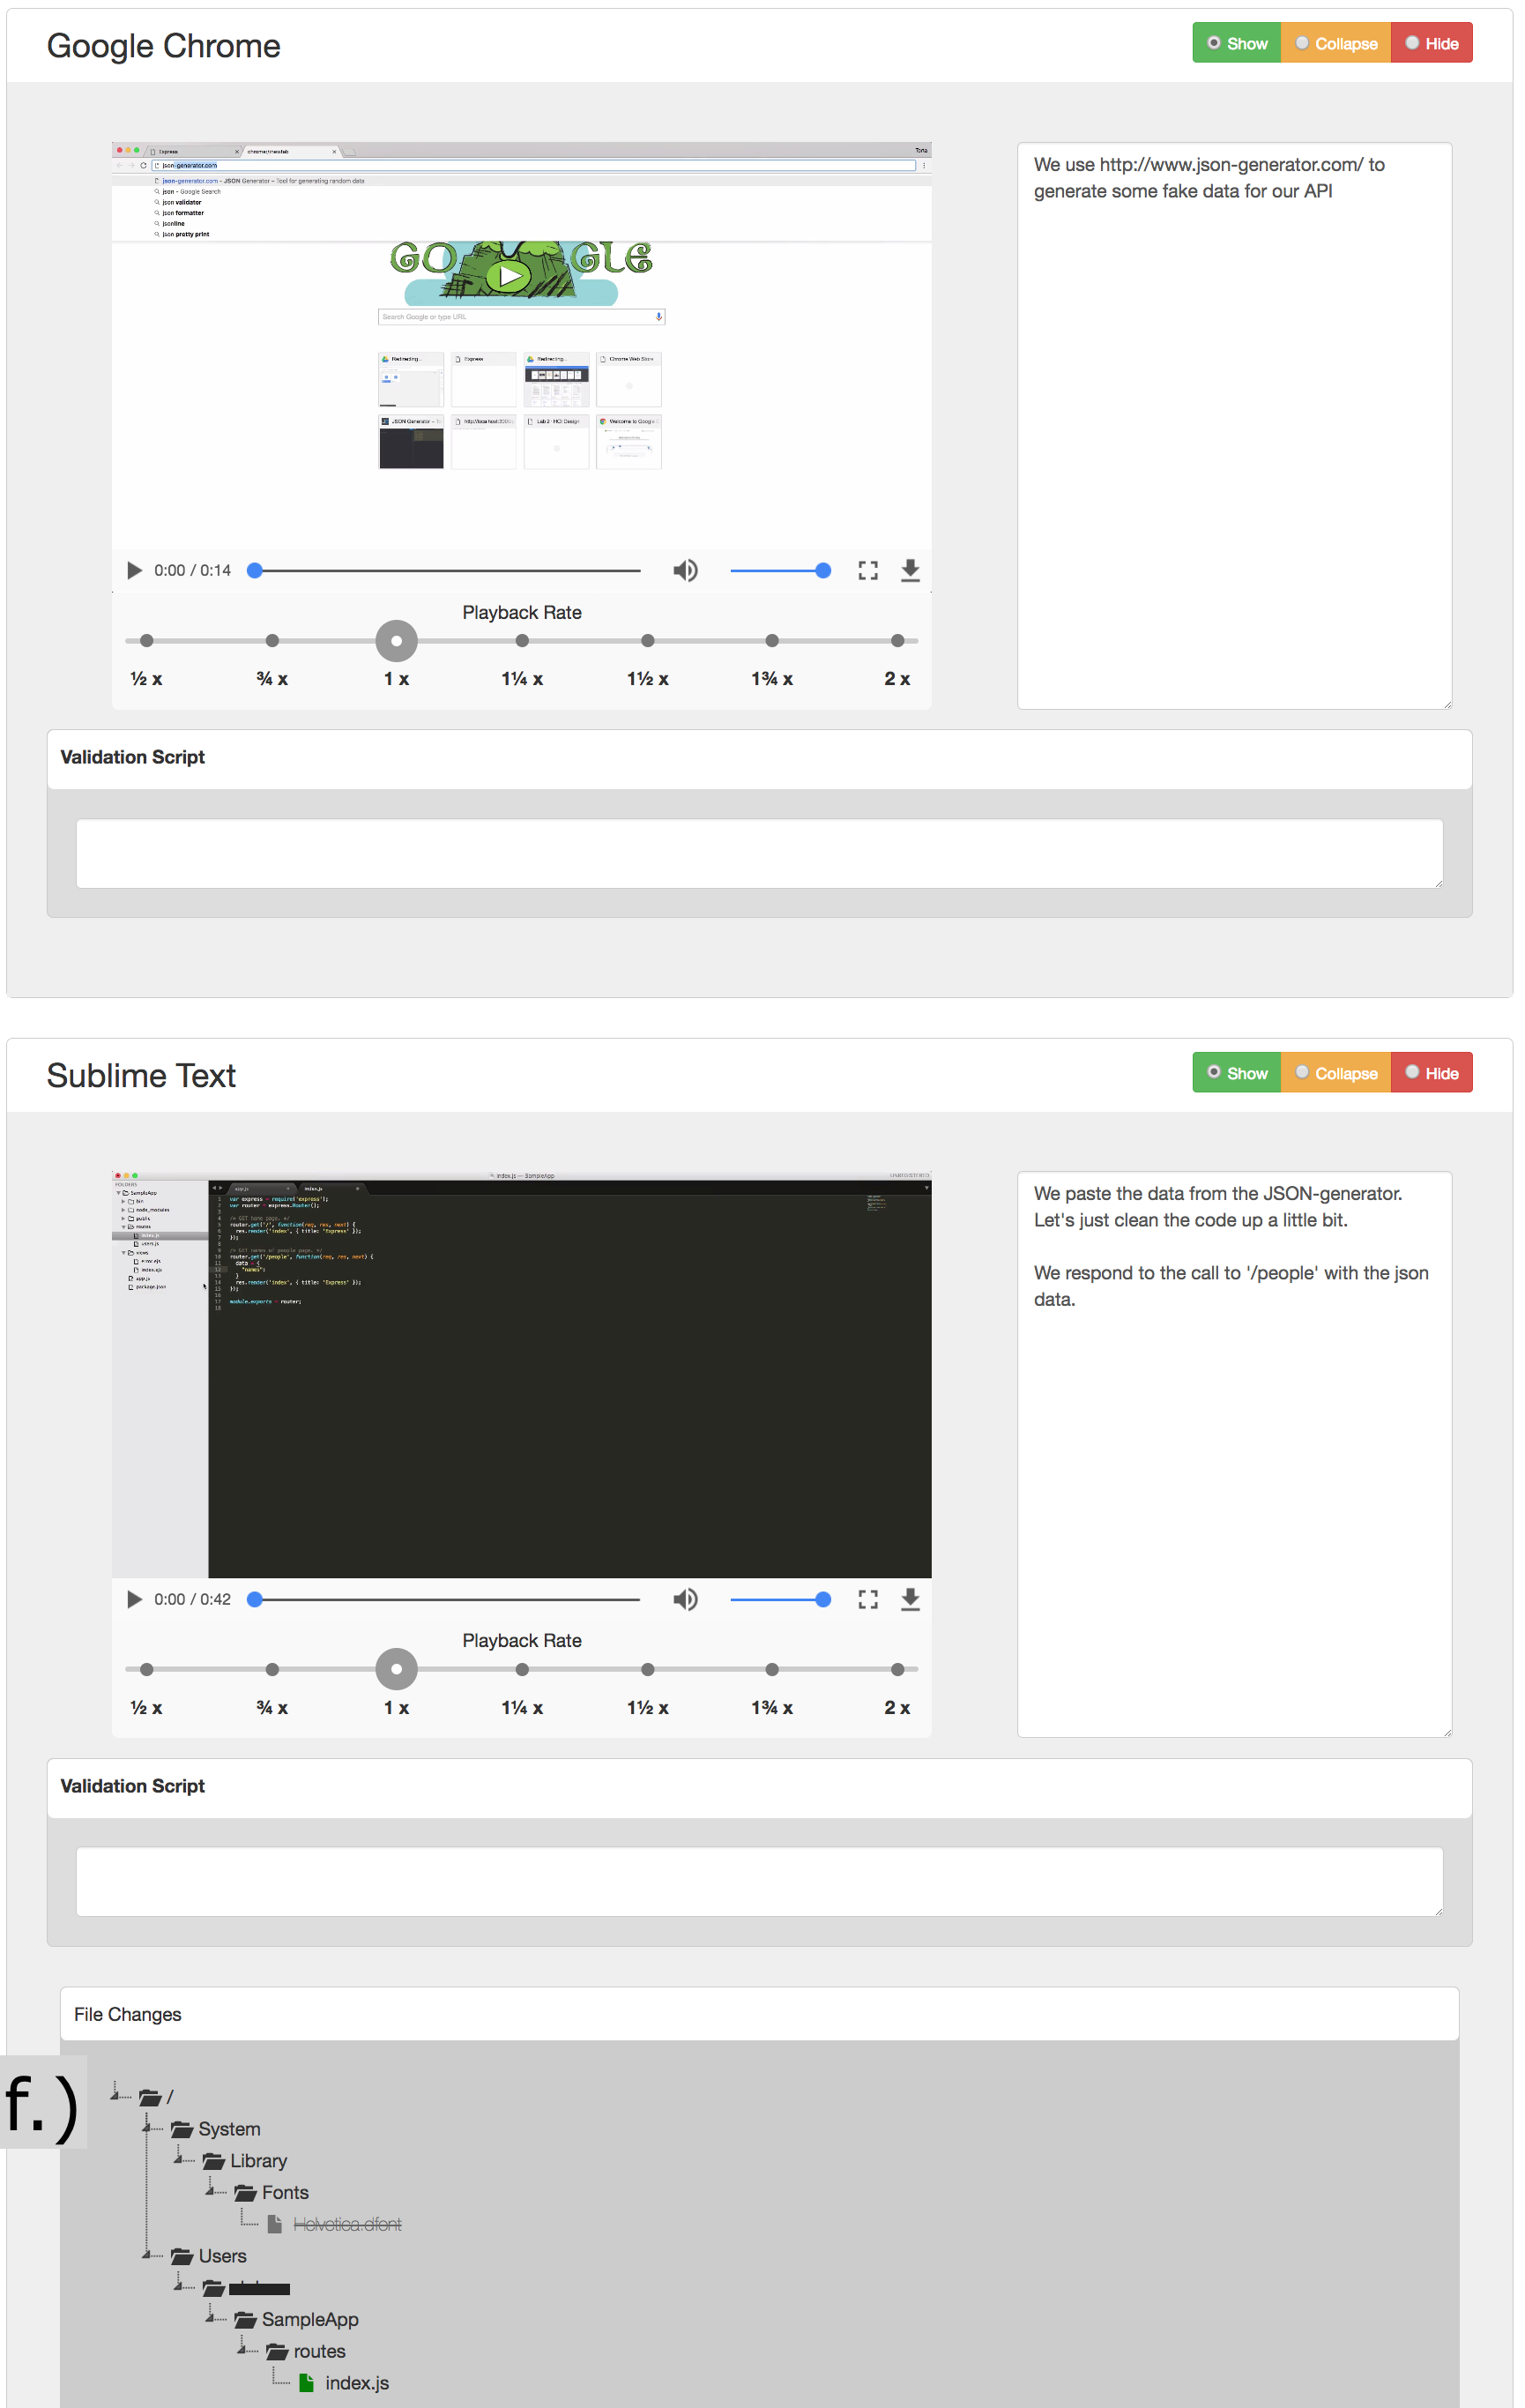
\includegraphics[width=0.362\textwidth]{figures/torta/editor-sublime-chrome.png}

\caption{Zoomed-in screenshots of Torta's tutorial editor showing three
steps (i.e., foreground windows): iTerm2, Google Chrome, and Sublime
Text. Each step contains:
a.)~Video player with playback speed adjuster,
b.)~Text annotation box,
c.)~Toggle to show/collapse/hide this entire step,
d.)~Toggle to show/collapse/hide each sub-step (here the hidden shell command
sub-steps are crossed-out),
e.)~Validation script,
f.)~Filesystem tree (see \fig{fig:torta-fstree}).}

\label{fig:torta-editor}
\end{figure*}


%Throughout testing, we did not observe any noticeable
%run-time slowdowns from these tracers. The one exception was that we
%originally used FSEvents and OpenSnoop to trace filesystem activity, but
%those ended up being too slow and memory-intensive. We quickly switched
%to DTrace, which was much faster since it was designed for
%efficiency~\cite{Cantrill2004}.

After the user finishes recording their demonstration and shuts down
Torta, it automatically creates a \emph{mixed-media tutorial} by
post-processing and combining the recorded data  into self-contained
package that contains all traces, segmented videos, and saved file
versions (Design Goal D2). As shown in \fig{fig:torta-schematic}, a
Torta-generated tutorial has a hierarchical structure that aims to
follow the design guidelines of Chi et al.~\cite{Chi2012}:


\textbf{Top-level steps -- foreground GUI windows}: A Torta tutorial is
an ordered list of top-level steps. Each step spans the duration of one
foreground GUI window. Torta uses FFmpeg~\cite{ffmpeg} to split the screencast video into
one mini-video per foreground window duration and crops those videos to
show only the foreground window. We felt that foreground windows were
the most natural step boundaries for these kinds of software
tutorials, since users often perform a set of actions within one window
(e.g., an IDE) and then switch to another window (e.g., Photoshop) to
perform the next set.

Each step is rendered as a mini-video along with a \emph{filesystem
tree} showing which files were added, deleted, renamed, and modified by
processes associated with the foreground GUI window during that step
(\fig{fig:torta-fstree}). We chose to visualize filesystem changes since
those represent the persistent effects of user actions within an
application. Regardless of what kind of app the user is running, if some
action has a lasting effect on their computer, it will likely manifest
in the filesystem.


\textbf{Sub-steps}: Torta further splits each top-level step into
sub-steps based on two common kinds of user actions
(\fig{fig:torta-schematic}):

\begin{itemize}\itemsep0pt

\item \emph{\textbf{Shell commands}}: If the user runs multiple shell commands
within the duration of one foreground window (usually some kind of
terminal app), Torta splits that step into one sub-step for each command.
Each sub-step is shown as a mini-video spanning the duration of only
that command, the text of that command, its current working directory,
environment variables, and a filesystem tree showing what files that
command added, deleted, renamed, and modified.

\item \emph{\textbf{File saves}}: When the foreground window is an
interactive app such as an IDE, web browser, or image editor, the user
may be editing files and periodically saving their progress to disk.
Torta splits each step into sub-steps based on file save events,
treating saves like user-defined checkpoints in the tutorial. Again,
each sub-step gets its own mini-video. If the saved file is plain text,
Torta also shows the diffs between the current and previously-saved
versions, which is useful for showing edits in code and configuration
files. 

%\todo{how does Torta differentiate these file saves from the files
%mutated by a shell command shown above?!?}

\end{itemize}

%Torta bundles the entire tutorial -- all filtered traces, segmented
%videos, and saved file versions -- into a self-contained package that
%can be deployed to the web (Design Goal D2).


\subsection{Tutorial Editor}

The mixed-media tutorial that Torta automatically generates from the
user's demonstration is already complete and ready to view on the web.
One can think of it as a screencast video that is segmented and
enhanced with OS-level trace data. However, it can be hard
for users to record a pristine, error-free video in one take.
Furthermore, users also want to augment tutorials with textual
annotations and other customizations. To fulfill these needs, Torta
provides a tutorial editor,
%
which renders the tutorial just as the viewer would see it but
adds extra controls for the following actions (\fig{fig:torta-editor}):

\textbf{Adding text annotations to steps/sub-steps}: The user
should already provide audio narration when recording their
demonstration, which will show up in the screencast video. The editor
also lets them add Markdown-based rich-text annotations next to the segmented video for
each step/sub-step.
%These annotations support Markdown, which is useful
%for adding web links.
%
%In the future, we could hook Torta to an automated or crowd-based
%transcription service to automatically convert audio narration into
%textual annotations.

\textbf{Hiding steps/sub-steps}: The user can hide any step/sub-step
from the viewer to eliminate mistakes or redundancies (effectively
deleting them from the edited tutorial). If the user hides a step that
is in between two steps that belong to the same application, then those
two surrounding steps get merged into one. This happens when, say, the
user is in an IDE, then switches to a web browser to look up something
quickly, then switches back to the IDE. If the user hides the web
browser step because they deem it irrelevant for the tutorial, then the
two IDE steps get merged together as one step in the viewer.
%
\rev{Torta does not support post-hoc re-recording of steps in the
editor. A workaround is to record an entire session even with errors
included and then hide erroneous steps using the editor.}

%(Note that we did not implement reordering of steps since it rarely
%makes sense to change the order of actions within a software tutorial.)

\textbf{Collapsing steps/sub-steps}: If the user deems certain steps or
sub-steps to be less important for the tutorial, they can show them in a
collapsed form. The viewer will see those steps as a collapsed summary
but can manually un-collapse them to dive into details. Torta displays
compact summaries so that viewers can more easily skim step contents
(e.g., ``Photoshop window active for 2 minutes, modified 3 files").

Torta implements heuristics to automatically collapse certain
steps/sub-steps that are likely to be less important to the tutorial.
For instance, if a shell command does not make any changes to the
filesystem (e.g., {\small \texttt{ls}} or {\small \texttt{git status}}),
it is collapsed by default since the user was probably checking their
setup before proceeding to the next step. Also, if any GUI window was in
the foreground for less than 5 seconds, had less than 10 user
keystrokes, and did not modify the filesystem, then its step is also
collapsed by default. This filters out ``flickers" where the user
switches between windows momentarily to quickly check something before
the next step.
%
%Note that these also make good candidates for deletion, but it is up to
%the user to make the final decision to delete.

\begin{figure}[h!]

\centering
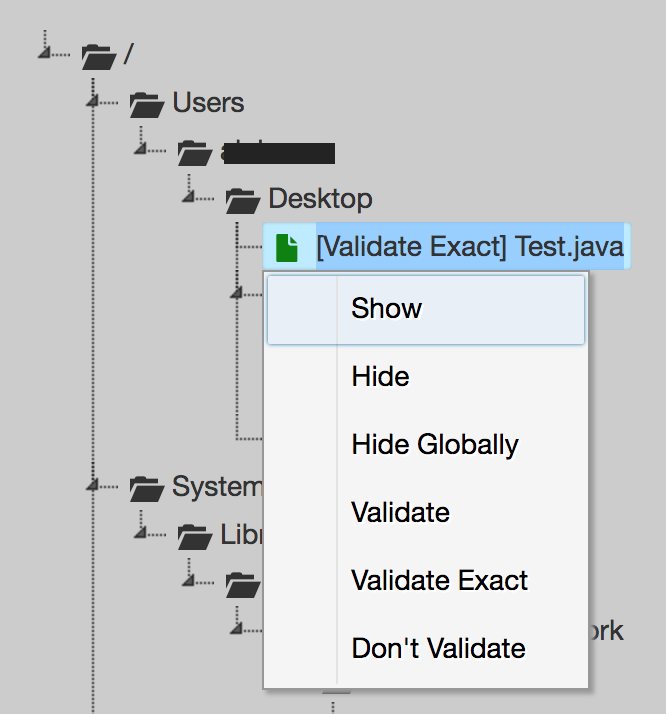
\includegraphics[width=0.56\columnwidth]{figures/torta/filesystem-tree.png}

\caption{Each file-modifying tutorial step displays a filesystem tree of
all files affected by running that step. In the editor UI, the user can
right-click to show/hide files and to mark for validation.}

\label{fig:torta-fstree}
\vspace{-0.5em} % stent
\end{figure}


\textbf{Collapsing filesystem tree components}: Recall that Torta
displays a filesystem tree within each step and
sub-step that modifies the filesystem (\fig{fig:torta-fstree}). However,
during pilot testing we
noticed that some commands (e.g., {\small \texttt{git clone}}) can
affect hundreds of files, so their trees are extremely large. To reduce
visual overload, the user can collapse tree nodes to hide and summarize
their sub-trees. For instance, the user can
collapse a {\small \texttt{.git/}} sub-directory to see a summary like
``100 files added and 15 files modified in \texttt{.git/}." Just as with
collapsed steps, the viewer can un-collapse tree nodes to see more details
on demand. The user can also choose ``Hide Globally" to hide a
particular file/directory across all tutorial steps.

%\textbf{Changing video playback speed}: Users can adjust the default
%playback speed for each video from 0.5X to 2X.

%Viewers can override the defaults if desired.

\textbf{Adding validation}: The editor provides two ways to specify how
people (i.e., tutorial \emph{consumers}) can validate progress at each
step as they are following the tutorial (Design Goal D4):

\emph{\textbf{1.~Marking files to validate}}: The user can mark each
file in the filesystem tree of a step/sub-step as ``Validate",
``Validate Exact," or ``Don't Validate" (\fig{fig:torta-fstree}). If the user marks a directory,
everything within it also gets marked with that label. ``Validate" means
that Torta should check that the consumer's file gets altered in the way
that this step specifies (e.g., modified or renamed), and ``Validate
Exact" means that the new contents of the file should also exactly match
the saved version bundled in the tutorial package. For example, in a step where the consumer is supposed
to add their username to a section within a configuration file, that
file should be marked as ``Validate" to check that it has been modified,
but not ``Validate Exact" since everyone's username will be different.

\emph{\textbf{2.~Writing validation scripts}}: File-based validation
handles the most common uses, but if tutorial creators want more
flexibility, they can write a validation script for each
step/sub-step (\fig{fig:torta-editor}e). This is a Bash script that will run on the consumer's
machine to check that their OS state is as expected.

\rev{This feature is similar in spirit to the step-level validation
features offered by tutorial systems for other
domains~\cite{Fernquist2011,Pongnumkul2011}}.

After the user finishes editing the tutorial, they can publish it as a
webpage or send the self-contained package to viewers.


\subsection{Tutorial Viewer}

Since Torta tutorials are ordinary webpages, they can be viewed in any
browser. Each tutorial initially loads with certain steps/sub-steps
collapsed, certain file tree nodes collapsed, and each video playing at the
speed pre-set by the creator. However, the user can adjust any of those
settings. In addition, they can click on any file in the tutorial and
view/download the version of that file present during that respective
step (all versions are stored in the package). This ability to
selectively hide and show details was inspired by a challenge discovered
during formative interviews: Students preferred seeing varying levels of
detail depending on their expertise level (Design Goal D3). It is hard
to achieve this flexibility with raw screencast videos or PowerPoint
slides.

To make tutorials more readable, Torta canonicalizes all file paths
within command invocations and filesystem trees. For instance, when
Alice creates a tutorial, many of her file paths will contain {\small
\texttt{/home/alice}} if they are within her home directory. But when
Bob is viewing the tutorial, he would prefer to see paths starting with
{\small \texttt{/home/bob}} instead of {\small \texttt{/home/alice}}.
Torta canonicalizes paths by replacing the creator's home directory with
the \texttt{\$HOME} variable. Additionally, the creator can use the
tutorial editor to specify other path variables to replace. One use case
is specifying a \texttt{\$PROJECT\_ROOT} directory where all files
within a project should live. The tutorial viewer prompts the user to
enter their own preferred values for all of these variables and rewrites
all paths within the webpage accordingly. Note that \texttt{\$HOME} and
other environment variables are automatically set if the tutorial is
loaded from the user's machine rather than viewed on the web.


\begin{figure}[h!]

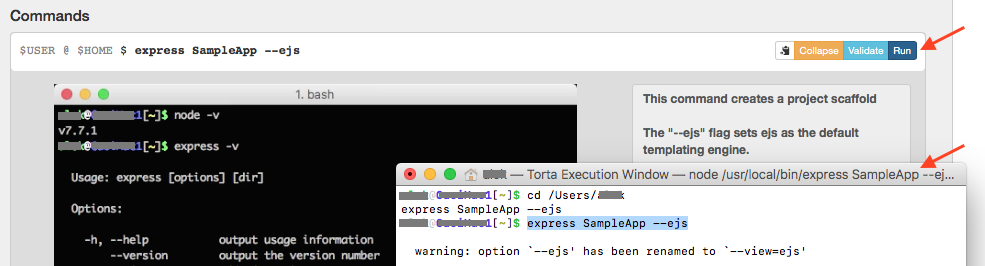
\includegraphics[width=\columnwidth]{figures/torta/view-and-run.png}

\caption{Each step and sub-step contains ``Validate" and ``Run" buttons
on the upper right. Here when the user clicks on ``Run" for a shell
command sub-step, Torta runs that commands in a new terminal window.}

\label{fig:torta-player}
\vspace{-1em} % stent
\end{figure}


If the user downloads the tutorial to their macOS machine and loads it
via the Torta viewer web app on localhost, then they can access two additional features as shown
in \fig{fig:torta-player}:

\emph{\textbf{1. Validating step-by-step progress}}: After manually
performing the actions specified by a particular step/sub-step, the user
can click the ``validate" button alongside its video. Torta will check
that the affected files on the user's local filesystem have been
modified in the ways that the creator originally expected (i.e.,
specified via ``validate" and ``validate exact" labels in the filesystem
tree) and also run the validation script if it exists. Then it prompts the user if
there are errors and offers to overwrite any mismatched files with
the versions from the tutorial package if the user wishes. This
capability lets the user check that they are properly following along
with each step of the tutorial and to catch bugs earlier (Design Goal
D4).

\emph{\textbf{2. Automatically running steps}}: The user can click the
``run" button next to each step/sub-step to have Torta automatically run
that step for them.  For a shell command, Torta launches a terminal
app on the user's machine and runs the command from that terminal after
setting the proper working directory and environment variables. For a
step involving a GUI application, Torta does not try to replay GUI
actions but rather simply mutates the user's filesystem in the way that
has been prescribed by that step. Although this approach is not
always guaranteed to be fully faithful to that step's actions, in practice it
works well in some cases since the persistent effects of a GUI
application usually manifest in the filesystem. For instance, if someone
demonstrates how to use a GUI to customize the configuration of a
complex interactive application, the effects of that customization
may show up as changes to some config file. When the user hits
``run" on that step, Torta simply copies over the updated version of that
config file.
